\subsection{DCF}

\subsubsection{Gedrag}
Om te weten of het DCF-signaal ontvangen wordt, wordt er een karakter geschreven op het LCD. Het DCF\_debug signaal wat van de DCF-controller komt, geeft aan of het DCF-signaal ontvangen wordt. Om te zorgen dat er niet steeds geschreven hoeft te worden of het signaal ontvangen wordt of niet, is er een buffer geimplementeerd die het signaal een klokslag onthoudt. Dus alleen als het signaal verandert, hoeft het subblok van de DCF te gaan schrijven.

\subsubsection{Functionaliteit}
Om duidelijk te maken hoe het subblok DCF\_lcd werkt, staat in figuur \ref{fig:FSMdcf} de FSM van het subblok.

\subsubsection{FSM}

\begin{figure}[h!]
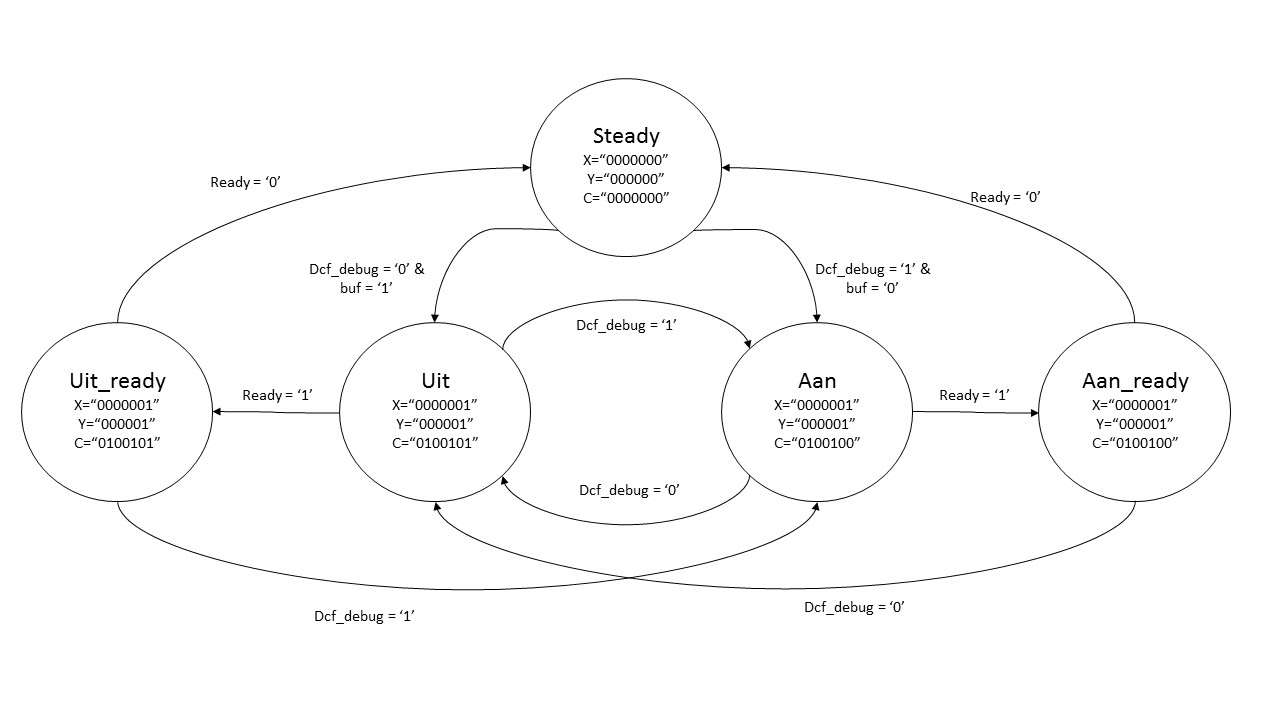
\includegraphics[width=15cm]{verslagschemas/FSMs/FSMdcf}
\caption{FSM van het subblok dcf\_lcd}
\label{fig:FSMdcf}
\end{figure}

\subsubsection{VHDL code}
De VHDL-code van het subblok \it{dcf\_lcd} staat in appendix \ref{code:beh_dcf-lcd}.

\subsubsection{Simulaties}
De resultaten van de simulatie aan het subblok \it{DCF\_lcd} is te vinden in appendix \ref{Ap:sim_LCD}
